\documentclass{article}
\usepackage[utf8]{inputenc}
\usepackage{setspace}
\usepackage{tikz}
\usetikzlibrary{positioning}
\usepackage{amsfonts}
\usepackage{amssymb}
\usepackage{amsmath}
\usepackage{amsthm}
\usepackage{systeme}
\usepackage{mathtools}
\usepackage{hyperref}

\begin{document}

\section*{Question 1}

~

\subsection*{Problem a}

~

\begin{equation*}
    \begin{split}
        &A^0=e=\begin{bmatrix}
            1&0\\
            0&1\\
        \end{bmatrix}\\
        &A^1=A=\begin{bmatrix}
            0&-1\\
            1&0\\
        \end{bmatrix}\\
        &A^2=\begin{bmatrix}
            0&-1\\
            1&0\\
        \end{bmatrix}\times\begin{bmatrix}
            0&-1\\
            1&0\\
        \end{bmatrix}=\begin{bmatrix}
            -1&0\\
            0&-1\\
        \end{bmatrix}\\
        &A^3=\begin{bmatrix}
            -1&0\\
            0&-1\\
        \end{bmatrix}\times\begin{bmatrix}
            0&-1\\
            1&0\\
        \end{bmatrix}=\begin{bmatrix}
            0&1\\
            -1&0\\
        \end{bmatrix}\\
        &A^4=\begin{bmatrix}
            0&1\\
            -1&0\\
        \end{bmatrix}\times\begin{bmatrix}
            0&-1\\
            1&0\\
        \end{bmatrix}=\begin{bmatrix}
            1&0\\
            0&1\\
        \end{bmatrix}=e\\
        \Rightarrow&\langle A\rangle=\left\{\begin{bmatrix}
            1&0\\
            0&1\\
        \end{bmatrix},\begin{bmatrix}
            0&-1\\
            1&0\\
        \end{bmatrix},\begin{bmatrix}
            -1&0\\
            0&-1\\
        \end{bmatrix},\begin{bmatrix}
            0&1\\
            -1&0\\
        \end{bmatrix}\right\}\\
    \end{split}
\end{equation*}

~

\subsection*{Problem b}

\begin{equation*}
    \begin{split}
        &z^0=e=1\\
        &e^1=z=\frac{1}{2}+\frac{\sqrt{3}}{2}i=e^{\frac{1}{3}\pi i}\\
        &e^2=e^{\frac{2}{3}\pi i}\\
        &e^3=e^{\pi i}\\
        &e^4=e^{\frac{4}{3}\pi i}\\
        &e^5=e^{\frac{5}{3}\pi i}\\
        &e^6=e^{2\pi i}=1=e\\
        &\langle z\rangle=\{1,e^{\frac{1}{3}\pi i},e^{\frac{2}{3}\pi i},e^{\pi i},e^{\frac{4}{3}\pi i},e^{\frac{5}{3}\pi i}\}\\
    \end{split}
\end{equation*}

\newpage

\section*{Question 2}

~

\subsection*{Problem a}

\begin{equation*}
    \begin{split}
        &U_k=\langle z\rangle\\
        &z^m=z^n \Leftrightarrow m\equiv n\mod k\\
        \Rightarrow&m\coloneqq ak+b,n\coloneqq ck+b,a,c\in\mathbb{Z} _{\geqslant 0},b\in[0,k)\cap\mathbb{Z}\\
        &f(z^m)=\begin{bmatrix}
            \cos(m\theta)&\sin(m\theta)\\
            -\sin(m\theta)&\cos(m\theta)\\
        \end{bmatrix}=\begin{bmatrix}
            \cos(\frac{(ak+b)2\pi}{k})&\sin(\frac{(ak+b)2\pi}{k})\\
            -\sin(\frac{(ak+b)2\pi}{k})&\cos(\frac{(ak+b)2\pi}{k})\\
        \end{bmatrix}=\begin{bmatrix}
            \cos(\frac{2b\pi}{k})&\sin(\frac{2b\pi}{k})\\
            -\sin(\frac{2b\pi}{k})&\cos(\frac{2b\pi}{k})\\
        \end{bmatrix}\\
        &f(z^n)=\begin{bmatrix}
            \cos(n\theta)&\sin(n\theta)\\
            -\sin(n\theta)&\cos(n\theta)\\
        \end{bmatrix}=\begin{bmatrix}
            \cos(\frac{(ck+b)2\pi}{k})&\sin(\frac{(ck+b)2\pi}{k})\\
            -\sin(\frac{(ck+b)2\pi}{k})&\cos(\frac{(ck+b)2\pi}{k})\\
        \end{bmatrix}=\begin{bmatrix}
            \cos(\frac{2b\pi}{k})&\sin(\frac{2b\pi}{k})\\
            -\sin(\frac{2b\pi}{k})&\cos(\frac{2b\pi}{k})\\
        \end{bmatrix}\\
        \Rightarrow&z^m=z^n\implies f(z^m)=f(z^n)\\
    \end{split}
\end{equation*}

~

\subsection*{Problem b}

~

\begin{equation*}
    \begin{split}
        &\cos(n\theta),\pm \sin(n\theta)\in\mathbb{R}\forall n,\theta\in\mathbb{R} \\
        \Rightarrow&\forall h\in H, h\in GL_2(\mathbb{R} )\\
        \Rightarrow&H\subseteq GL_2(\mathbb{R} )\\
        &\text{Identity}:\\
        &e\in GL_2(\mathbb{R} )=\begin{bmatrix}
            1&0\\
            0&1\\
        \end{bmatrix}\\
        &n=0\\
        \Rightarrow&f(z^0)=\begin{bmatrix}
            \cos(0)&\sin(0)\\
            -\sin(0)&\cos(0)\\
        \end{bmatrix}=\begin{bmatrix}
            1&0\\
            0&1\\
        \end{bmatrix}=e\\
        \Rightarrow&e\in H\\
        &\text{Inverse}:\\
        &f(z^n)=\begin{bmatrix}
            \cos(n\theta)&\sin(n\theta)\\
            -\sin(n\theta)&\cos(n\theta)\\
        \end{bmatrix}\\
        &(f(z^n))^{-1}\times f(n^z)=e\\
        \Rightarrow&(f(z^n))^{-1}\times\begin{bmatrix}
            \cos(n\theta)&\sin(n\theta)\\
            -\sin(n\theta)&\cos(n\theta)\\
        \end{bmatrix}=\begin{bmatrix}
            1&0\\
            0&1\\
        \end{bmatrix}\\
        \Rightarrow&(f(z^n))^{-1}=\begin{bmatrix}
            \cos(n\theta)&-\sin(n\theta)\\
            \sin(n\theta)&\cos(n\theta)\\
        \end{bmatrix}=\begin{bmatrix}
            \cos(-n\theta)&\sin(-n\theta)\\
            -\sin(-n\theta)&\cos(-n\theta)\\
        \end{bmatrix}=f(z^{-n})\\
        \Rightarrow&(f(z^n))^{-1}=f(z^{-n})\in H\\
    \end{split}
\end{equation*}

\begin{equation*}
    \begin{split}
        &\text{Closure}:\\
        &A\coloneqq f(z^m),B\coloneqq f(z^n)\\
        &A=\begin{bmatrix}
            \cos(m\theta)&\sin(m\theta)\\
            -\sin(m\theta)&\cos(m\theta)\\
        \end{bmatrix},B=\begin{bmatrix}
            \cos(n\theta)&\sin(n\theta)\\
            -\sin(n\theta)&\cos(n\theta)\\
        \end{bmatrix}\\
        &AB=\begin{bmatrix}
            \cos(m\theta)&\sin(m\theta)\\
            -\sin(m\theta)&\cos(m\theta)\\
        \end{bmatrix}\times \begin{bmatrix}
            \cos(n\theta)&\sin(n\theta)\\
            -\sin(n\theta)&\cos(n\theta)\\
        \end{bmatrix}\\
        \Rightarrow&AB=\begin{bmatrix}
            \cos(m\theta)\cos(n\theta)-\sin(n\theta)\sin(n\theta)&\cos(m\theta)\sin(n\theta)+\sin(m\theta)\cos(n\theta)\\
            -\sin(m\theta)\cos(n\theta)-\cos(m\theta)\sin(n\theta)&-\sin(m\theta)\sin(n\theta)+\cos(m\theta)\cos(n\theta)\\
        \end{bmatrix}\\
        &AB=\begin{bmatrix}
            \cos((m+n)\theta)&\sin((m+n)\theta)\\
            -\sin((m+n)\theta)&\cos((m+n)\theta)\\
        \end{bmatrix}=f(z^{m+n})\in H\\
        \Rightarrow&H\text{ is a subgroup}\\
    \end{split}
\end{equation*}

~

\subsection*{Problem c}

~

\begin{equation*}
    \begin{split}
        &\text{Injective}:\\
        &f(z^m)=f(z^n)\\
        &\begin{bmatrix}
            \cos(m\theta)&\sin(m\theta)\\
            -\sin(m\theta)&\cos(m\theta)\\
        \end{bmatrix}=\begin{bmatrix}
            \cos(n\theta)&\sin(n\theta)\\
            -\sin(n\theta)&\cos(n\theta)\\
        \end{bmatrix}\\
        \Rightarrow&m\theta\equiv n\theta \mod 2\pi\\
        \Rightarrow&m\equiv n\mod k\leftarrow\theta=\frac{2\pi}{k}\\
        \Rightarrow&z^m=z^n\in U_k\leftarrow\text{Problem a}\\
        \Rightarrow&f\text{ is injective}\\
        &\text{Surjective}:\\
        &\forall z^m\in U_k ,f(z^m)=\begin{bmatrix}
            \cos(m\theta)&\sin(m\theta)\\
            -\sin(m\theta)&\cos(m\theta)\\
        \end{bmatrix}\\
        &\forall m\in\mathbb{Z} ,\exists n\in[0,k)\in\mathbb{Z} :m\equiv n\mod k\\
        \Rightarrow&\forall z^m\in U_k,\begin{bmatrix}
            \cos(m\theta)&\sin(m\theta)\\
            -\sin(m\theta)&\cos(m\theta)\\
        \end{bmatrix}=\begin{bmatrix}
            \cos(n\theta)&\sin(n\theta)\\
            -\sin(n\theta)&\cos(n\theta)\\
        \end{bmatrix}\in H\\
        \Rightarrow&f\text{ is surjective}\\
    \end{split}
\end{equation*}

\begin{equation*}
    \begin{split}
        &\text{Homomorphism}:\\
        &AB=f(z^{m+n})\leftarrow \text{Problem b}\\
        &A=f(z^m),B=f(z^n)\\
        \Rightarrow&f(z^{m+n})=f(z^m)f(z^n)\\
        \Rightarrow&f(z^mz^n)=f(z^m)f(z^n)\\
        \Rightarrow&f\text{ is isomorphic}\\
    \end{split}
\end{equation*}

\newpage

\section*{Question 3}

~

\begin{equation*}
    \begin{split}
        &\det (A)\ne 1\\
        \Rightarrow&\det(A^n)\ne1\forall n\ne 0\in \mathbb{Z} \\
        \Rightarrow&\nexists n\ne 0\in \mathbb{Z}:A^n=e\\
        &\langle A\rangle\text{ is infinite}\\
        &\langle A\rangle\text{ is generated by }A\\
        \Rightarrow&\langle A\rangle\text{ is a cyclic group by definition}\\
        \Rightarrow&\langle A\rangle\cong \begin{cases*}
            \langle\mathbb{Z} ,+\rangle,|\langle A\rangle|=\infty\\
            \langle\mathbb{Z} ,+_k\rangle,|\langle A\rangle|=k,k\in\mathbb{Z} _{>0}\\
        \end{cases*}\\
        \Rightarrow&\langle A\rangle\cong \langle\mathbb{Z} ,+\rangle\\
    \end{split}
\end{equation*}

\newpage

\section*{Question 4}

~

\begin{equation*}
    \begin{split}
        &\text{Identity}:\\
        &\exists a\in G,a \sim a=a^{-1}a=e\\
        \Rightarrow&e\in H\\
        &\text{Inverse}:\\
        &\exists a\in H:a\in G,a\sim e\implies a^{-1}e =a^{-1}\in H\\
        &\text{Closure}:\\
        &\exists a,b\in H\\
        \Rightarrow&a^{-1}\in H\\
        \Rightarrow&a^{-1}\sim b\implies (a^{-1})^{-1}b=ab\in H\\
        \Rightarrow&a,b\in H\implies ab\in H\\
        \Rightarrow&a\sim b\implies H\text{ is a subgroup}\\
    \end{split}
\end{equation*}

\newpage

\section*{Question 5}

~

\subsection*{Problem a}

~

\begin{equation*}
    \begin{split}
        &\forall x\in\mathbb{Z} ,\exists! q\in\mathbb{Z} \land r\in[0,n)\cap\mathbb{Z} :x=nq+r,n \in \mathbb{Z} _{>0}\\
        &r\in\{0,1,2,...,n-1\}\\
        &|\{0,1,2,...,n-1\}|=n\\
        \Rightarrow&n\text{ different equivalence classes}\\
        &\forall x\in\mathbb{Z} ,\exists !r\in[0,n)\cap\mathbb{Z}:n-r=nq\\
        \Rightarrow&\forall x\in\mathbb{Z} ,x\in \overline{r}\in\{\overline{0},\overline{1},\overline{2},...,\overline{n-1}\}\\
        \Rightarrow&\text{There are exactly }n\text { equivalent classes}:\overline{0},\overline{1},\overline{2},...,\overline{n-1}\\
    \end{split}
\end{equation*}

~

\subsection*{Problem b}

~

\begin{equation*}
    \begin{split}
        &\overline{c_1}\coloneqq C_1,c_1\in[0,n)\cap\mathbb{Z}\\
        &\overline{c_2}\coloneqq C_2,c_2\in[0,n)\cap\mathbb{Z}\\
        &x_1\in C_1\implies x_1=k_1n+c_1,k_1\in \mathbb{Z} \\
        &x_2\in C_2\implies x_2=k_2n+c_2,k_2\in \mathbb{Z} \\
        &x_1+x_2=k_1n+c_1+k_2n+c_2=(c_1+c_2)+(k_1+k_2)n\sim c_1+c_2\\
        &\text{The result is inpendent of }k_1,k_2\\
        \Rightarrow&\forall x_1\in C_1,x_2\in C_2:x_1+x_2\sim c_1+c_2\\
        &C_1+C_2=\overline{x_1+x_2}\text { is well defined}\\
    \end{split}
\end{equation*}

~

\subsection*{Problem c}

~

\begin{equation*}
    \begin{split}
        &\text{Closure}:\\
        &\exists a,b\in[0,n)\cap\mathbb{Z} ,A\coloneqq \overline{a},B\coloneqq \overline{b}\in S\\
        \Rightarrow&A+B=\overline{a+b}\leftarrow\text{Problem b}\\
        &a,b\in[0,n)\cap\mathbb{Z}\implies a+b\in[0,2n)\cap\mathbb{Z}\\
        &a+b=\begin{cases*}
            a+b,a+b\in[0,n)\cap\mathbb{Z}\\
            a+b-n,a+b\in[n,2n)\cap\mathbb{Z}\\
        \end{cases*}\\
        \Rightarrow&a+b\in[0,n)\cap\mathbb{Z}\\
        \Rightarrow&\overline{a+b}\in S\\
        &\text{Identity}:\\
        &\exists \overline{a}\in S\\
        &\overline{a}+\overline{0}=\overline{a+0}=\overline{a}\in S\\
        \Rightarrow&e=\overline{0}\in S\\
        &\text{Inverse}:\\
        &\exists \overline{a}\in S\\
        &\overline{a}+\overline{n-a}=\overline{a+n-a}=\overline{n}=\overline{0}\in S\\
        \Rightarrow&\forall\overline{a}\in S,\exists \overline{n-a}\in S:\overline{a}+\overline{n-a}=e\\
        &\text{Associativity}:\\
        &\exists \overline{a},\overline{b},\overline{c}\in S\\
        &(\overline{a}+\overline{b})+\overline{c}=\overline{a+b}+\overline{c}=\overline{a+b+c}\\
        &\overline{a}+(\overline{b}+\overline{c})=\overline{a}+\overline{b+c}=\overline{a+b+c}\\
        \Rightarrow&(\overline{a}+\overline{b})+\overline{c}=\overline{a}+(\overline{b}+\overline{c})\\
        \Rightarrow&S\text{ is a group}\\
        &\overline{1}\in S\\
        &\forall k\in\mathbb{Z} _{>0}:\overline{k}=\underbrace{\overline{1}+\overline{1}+\overline{1}+...+\overline{1}}_{k\text{ times}}\\
        &\overline{0}=\overline{n}=\underbrace{\overline{1}+\overline{1}+\overline{1}+...+\overline{1}}_{n\text{ times}}\\
        \Rightarrow&\overline{1}\text { can generate all the elements in }S\\
        \Rightarrow&\overline{1}\text{ is a generator of }\langle S,+\rangle\\
        &S\text{ is cyclic}\\
    \end{split}
\end{equation*}

\newpage

\section*{Question 6}

~

\subsection*{Problem a}

~

\begin{equation*}
    \begin{split}
        &\text{False}\\
        &\mathbb{Z} _5\\
        &\langle1\rangle=\langle2\rangle=\langle3\rangle=\langle4\rangle=\mathbb{Z} _5\\
        &\text{The generator is not unique for }\mathbb{Z} _5\\
    \end{split}
\end{equation*}

~

\subsection*{Problem b}

~

\begin{equation*}
    \begin{split}
        &\text{False}\\
        &\mathbb{Z}_4\\
        &\langle2\rangle=\{0,2\}\ne\mathbb{Z}_4\\
        &\text{Not all elements in a cyclic group is a generator}\\
    \end{split}
\end{equation*}

~

\subsection*{Problem c}

~

\begin{equation*}
    \begin{split}
        &\text{False}\\
        &\text{Consider }\mathbb{V}_4:\\
        &\begin{array}{c|cccc}
            \ast&e&a&b&c\\
            \hline
            e&e&a&b&c\\
            a&a&e&c&b\\
            b&b&c&e&a\\
            c&c&b&a&e\\
        \end{array}\\
        \Rightarrow&e^2=a^2=b^2=c^2=e\\
    \end{split}
\end{equation*}

~

\subsection*{Problem d}

~

\begin{equation*}
    \begin{split}
        &\text{True}\\
        &\text{All cyclic groups are isomorphic to }\mathbb{Z} \text{ or }\mathbb{Z} _n\\
        &\mathbb{Z} :\\
        &\mathbb{Z}=\langle a\rangle=\{...,a^{-2},a^{-1},e,a^{1},a^{2},...\}\\
        &\langle a\rangle\text{ is infinite}\implies \forall n\in Z,\nexists m\ne e\in \langle a\rangle:a^n=e\\
        \Rightarrow& a^2=e\implies a=e\leftarrow\text{unique solution}\\
        &\mathbb{Z} _n:\\
        &a^2=e\Leftrightarrow 2a\equiv 0\mod n\\
        &\forall a\in [0,n),2a\in [0,2n)\\
        \Rightarrow&2a\equiv 0\mod n\implies 2a=0\lor 2a=n\\
        &2|n:\\
        &a=0\lor a=n\\
        &\text{two solutions}\\
        &2|n+1:\\
        &a=0\\
        &\text{unique solution}\\
        \Rightarrow&\text{at most two solutions}\\
    \end{split}
\end{equation*}

~

\subsection*{Problem e}

~

\begin{equation*}
    \begin{split}
        &\text{True}\\
        &n=1:\text{group is trivial}\\
        &n>1:\exists \mathbb{V} _n\text{ as a group of order }n\\
        &\mathbb{V}_n\text{ is abelian}\\
    \end{split}
\end{equation*}

~

\subsection*{Problem f}

~

\begin{equation*}
    \begin{split}
        &g\in G\\
        \Rightarrow&g^{-1}\in G\\
        &G\text{ has only one gneerator}:\\
        \Rightarrow&g=g^{-1}\\
        \Rightarrow&g^{2}=e\\
        \Rightarrow&G=\{e,g\}=\langle g\rangle\\
    \end{split}
\end{equation*}

\newpage

\section*{Question 7}

~

\subsection*{Problem a}

~

\begin{equation*}
    \begin{split}
        &\langle0\rangle=\{0\}\\
        &\langle1\rangle=\{0,1,2,3,4,5,6,7\}=\mathbb{Z} _8\\
        &\langle2\rangle=\{0,2,4,6\}\\
        &\langle3\rangle=\{0,1,2,3,4,5,6,7\}=\mathbb{Z} _8\\
        &\langle4\rangle=\{0,4\}\\
        &\langle5\rangle=\{0,1,2,3,4,5,6,7\}=\mathbb{Z} _8\\
        &\langle6\rangle=\{0,2,4,6\}\\
        &\langle7\rangle=\{0,1,2,3,4,5,6,7\}=\mathbb{Z} _8\\
    \end{split}
\end{equation*}

~

\subsection*{Problem b}

~

\begin{equation*}
    \begin{split}
        &\langle1\rangle=\{0,1,2,3,4,5,6,7\}=\mathbb{Z} _8\\
        &\langle3\rangle=\{0,1,2,3,4,5,6,7\}=\mathbb{Z} _8\\
        &\langle5\rangle=\{0,1,2,3,4,5,6,7\}=\mathbb{Z} _8\\
        &\langle7\rangle=\{0,1,2,3,4,5,6,7\}=\mathbb{Z} _8\\
        \Rightarrow&1,3,5,7\text{ are the generators of the group}\\
    \end{split}
\end{equation*}

\newpage

\section*{Question 8}

~

\begin{equation*}
    \begin{split}
        &\mathbb{Z} _5:\\
        &\langle1\rangle=\langle2\rangle=\langle3\rangle=\langle4\rangle=\mathbb{Z}_5\\
        &\langle0\rangle=\{0\}\\
    \end{split}
\end{equation*}

\begin{figure}[!ht]
    \centering
    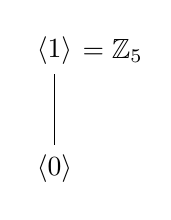
\begin{tikzpicture}[node distance=1.5cm]
        \node(A1)  {$\langle 1 \rangle$};
        \node(A2) [below of= A1] {$\langle 0 \rangle$};
        \node[right=0pt of A1,inner xsep=0pt] {$= \mathbb{Z}_{5}$};
        \draw(A1) -- (A2);
    \end{tikzpicture}
\end{figure}

\begin{equation*}
    \begin{split}
        &\mathbb{Z} _6:\\
        &\langle1\rangle=\langle5\rangle=\mathbb{Z}_6\\
        &\langle2\rangle=\langle4\rangle=\{0,2,4\}\\
        &\langle3\rangle=\{0,3\}\\
        &\langle0\rangle=\{0\}\\
    \end{split}
\end{equation*}

\begin{figure}[!ht]
    \centering
    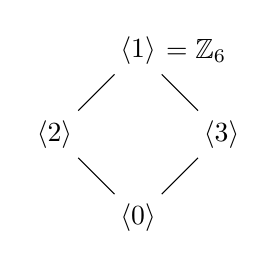
\begin{tikzpicture}[node distance=1.5cm]
        \node(A1)  {$\langle 1 \rangle$};
        \node(A2) [below left of= A1] {$\langle 2 \rangle$};
        \node(A3) [below right of= A1] {$\langle3\rangle$};
        \node(A4) [below right of= A2] {$\langle0\rangle$};
        \node[right=0pt of A1,inner xsep=0pt] {$= \mathbb{Z}_{6}$};
        \draw(A1) -- (A2);
        \draw(A1) -- (A3);
        \draw(A2) -- (A4);
        \draw(A3) -- (A4);
    \end{tikzpicture}
\end{figure}

\begin{equation*}
    \begin{split}
        &\mathbb{Z} _8:\\
        &\langle1\rangle=\langle3\rangle=\langle5\rangle=\langle7\rangle=\mathbb{Z}_8\\
        &\langle2\rangle=\langle6\rangle=\{0,2,4,6\}\\
        &\langle4\rangle=\{0,4\}\\
        &\langle0\rangle=\{0\}\\
    \end{split}
\end{equation*}

\newpage

\begin{figure}[!ht]
    \centering
    \begin{tikzpicture}[node distance=1.5cm]
        \node(A1)  {$\langle 1 \rangle$};
        \node(A2) [below  of= A1] {$\langle 2 \rangle$};
        \node(A3) [below  of= A2] {$\langle4\rangle$};
        \node(A4) [below  of= A3] {$\langle0\rangle$};
        \node[right=0pt of A1,inner xsep=0pt] {$= \mathbb{Z}_{8}$};
        \draw(A1) -- (A2);
        \draw(A2) -- (A3);
        \draw(A3) -- (A4);
    \end{tikzpicture}
\end{figure}

\begin{equation*}
    \begin{split}
        &\mathbb{Z} _{12}:\\
        &\langle1\rangle=\langle5\rangle=\langle7\rangle=\langle11\rangle=\mathbb{Z}_{12}\\
        &\langle2\rangle=\langle10\rangle=\{0,2,4,6,8,10\}\\
        &\langle3\rangle=\langle9\rangle=\{0,3,6,9\}\\
        &\langle4\rangle=\langle8\rangle=\{0,4,8\}\\
        &\langle6\rangle=\{0,6\}\\
        &\langle0\rangle=\{0\}\\
    \end{split}
\end{equation*}

\begin{figure}[!ht]
    \centering
    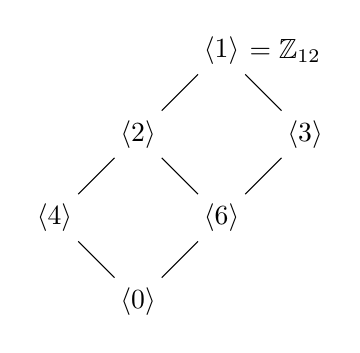
\begin{tikzpicture}[node distance=1.5cm]
        \node(A1)  {$\langle 1 \rangle$};
        \node(A2) [below left of= A1] {$\langle 2 \rangle$};
        \node(A3) [below right of= A1] {$\langle3\rangle$};
        \node(A4) [below left of= A3] {$\langle6\rangle$};
        \node(A5) [below left of= A2] {$\langle4\rangle$};
        \node(A6) [below left of= A4] {$\langle0\rangle$};
        \node[right=0pt of A1,inner xsep=0pt] {$= \mathbb{Z}_{12}$};
        \draw(A1) -- (A2);
        \draw(A1) -- (A3);
        \draw(A2) -- (A4);
        \draw(A3) -- (A4);
        \draw(A2) -- (A5);
        \draw(A4) -- (A6);
        \draw(A5) -- (A6);
    \end{tikzpicture}
\end{figure}

\newpage

\section*{Question 9}

\begin{equation*}
    \begin{split}
        &G\ne\{e\}\\
        \Rightarrow&g\ne e\in G\\
        \Rightarrow&\langle g\rangle\subseteq G\\
        &\langle g\rangle\ne\{e\}\\
        \Rightarrow&\langle g\rangle=G\\
        \Rightarrow&G\text{ is cyclic}\\
        &\langle g^2\rangle =\{e\}\lor \langle g^2\rangle =G=\langle g\rangle\\
        &\langle g^2\rangle =\{e\}\implies |G|=2\\
        &\langle g^2\rangle =G=\langle g\rangle:\\
        &\exists k\in \mathbb{Z} :g^{2k}=g\\
        \Rightarrow&e=g^{2k-1}\\
        &|G|\coloneqq m\\
        &\exists h\in(1,n)\in\mathbb{Z} :\langle g^h\rangle=\langle g\rangle\\
        \Rightarrow&\exists n\in\mathbb{Z} g^{nh}=g\\
        &g^{nh-1}=e\\
        \Rightarrow&m|nh-1\\
        \Rightarrow&\gcd(m,h)=1\forall h\in(1,n)\\
        \Rightarrow&m\text{ is prime}\\
    \end{split}
\end{equation*}

\newpage

\section*{Question 10}

\begin{equation*}
    \begin{split}
        &\langle\mathbb{Z},+_5\rangle\\
        &|\langle\mathbb{Z},+_5\rangle|=5\\
        &\langle\mathbb{Z} ,+_5\rangle=\langle1\rangle=\langle2\rangle=\langle3\rangle=\langle4\rangle\\
        &\langle\mathbb{Z} ,+_8\rangle\\
        &|\langle\mathbb{Z} ,+_8\rangle|=8\\
        &\langle\mathbb{Z} ,+_8\rangle=\langle1\rangle=\langle3\rangle=\langle5\rangle=\langle7\rangle\\
        &\langle\mathbb{Z} ,+_{10}\rangle\\
        &|\langle\mathbb{Z} ,+_{10}\rangle|=10\\
        &\langle\mathbb{Z} ,+_{10}\rangle=\langle1\rangle=\langle3\rangle=\langle7\rangle=\langle9\rangle\\
    \end{split}
\end{equation*}
\end{document}